%% ---------------------------------------------------------------------------------------------------------------------

\chapter{\textit{go-safer}: Detecting Unsafe Misuses}\label{ch:go-safer}

Another major contribution of this thesis is the development of a Go Vet-style, open-source linter tool.
It can identify some of the unsafe code patterns.

\begin{figure}[htp!]
    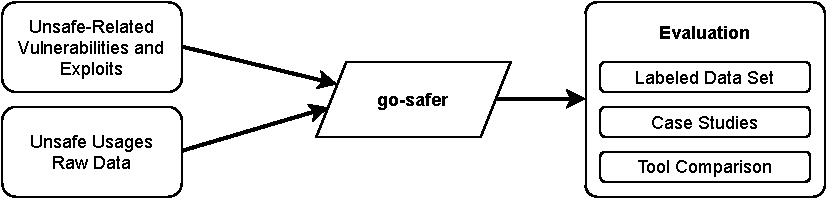
\includegraphics[width=\textwidth]{assets/figures/chapter5/outline5.pdf}
    \caption{Role of Chapter 5 in the thesis outline}
    \label{fig:outline5}
\end{figure}



%% ---------------------------------------------------------------------------------------------------------------------

\section{Design}\label{sec:go-safer:design}

%Top-level approach
%Usage example
%Publication

\begin{figure}[!t]
    \vspace{2mm}
    \centering
    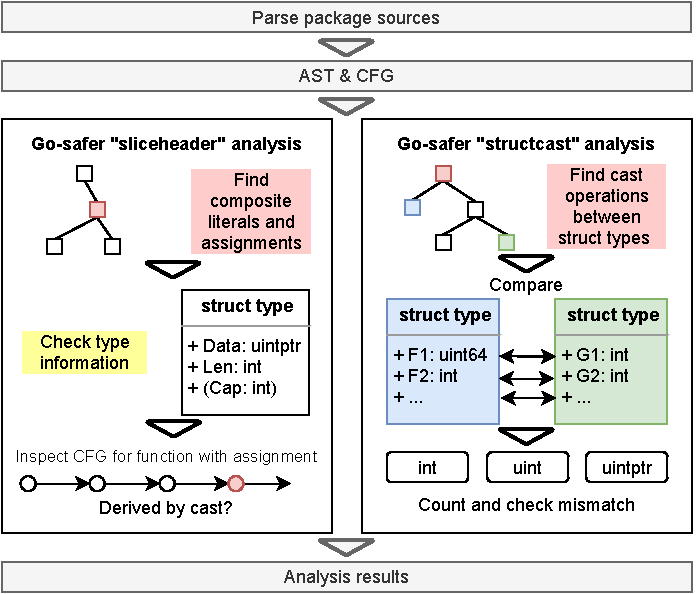
\includegraphics[width=0.48\textwidth]{gfx/figures/go-safer-architecture.pdf}
    %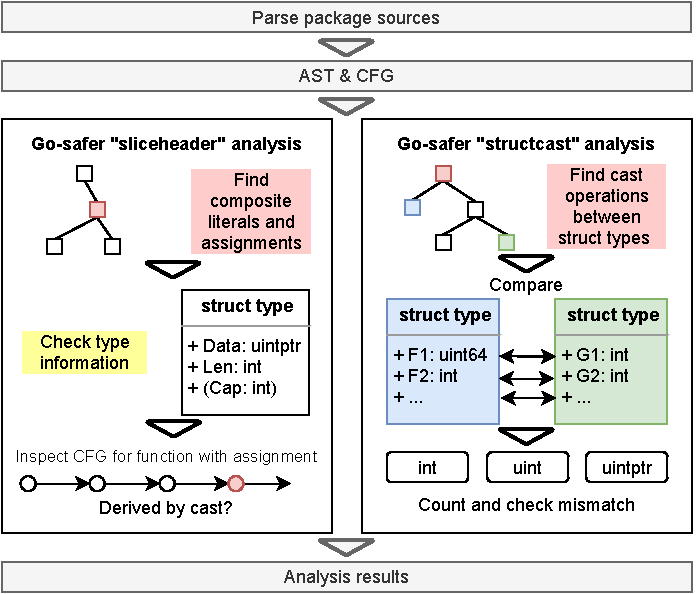
\includegraphics[width=0.45\textwidth]{gfx/figures/go-safer-architecture.pdf}
    \caption{Architecture of \toolSA{} static code analysis tool}
    \label{fig:safer-architecture}
    %\vspace{-14pt}
\end{figure}



%% ---------------------------------------------------------------------------------------------------------------------

\section{Implementation}\label{sec:go-safer:implementation}

%Go vet analysis pass infrastructure
%Low-level details
%Verification with tests


%% ---------------------------------------------------------------------------------------------------------------------

\section{Evaluation}\label{sec:go-safer:evaluation}


%% ---------------------------------------------------------------------------------------------------------------------

\subsection{Labeled Usages}\label{subsec:go-safer:evaluation:labeled-usages}

%Precision, Recall, calculated using manually labeled usages data set


%% ---------------------------------------------------------------------------------------------------------------------

\subsection{Case Studies}\label{subsec:go-safer:evaluation:case-studies}

%Manual inspection of some projects, used to calculate precision / recall of go-safer


%% ---------------------------------------------------------------------------------------------------------------------

\subsection{Comparison with Existing Tools}\label{subsec:go-safer:evaluation:linters-comparison}

%Go vet / Gosec
